\documentclass[11pt]{article}

\usepackage{sectsty}
\usepackage{graphicx}
\usepackage{hyperref}
\hypersetup{ colorlinks=true, urlcolor=blue}

\usepackage{wrapfig}

% Margins
\topmargin=-0.45in
\evensidemargin=0in
\oddsidemargin=0in
\textwidth=6.5in
\textheight=9.0in
\headsep=0.25in


\usepackage{xcolor}

\newcommand{\todo}[1]{\color{red}{\colorbox{pink}{\textbf{#1}}}\color{black}}



\title{DATA 200 Graduate Project\\ {\Large Topic 1: COVID-19}\\
{\large Dataset A: Testing \& Mortality Statistics}}
\author{ Anya Michaelsen (SID 3034964414) }
\date{}

\begin{document}
\maketitle	
%\pagebreak

% Optional TOC
{ \hypersetup{hidelinks} \tableofcontents }% \pagebreak

%--Paper--

%\section{Report Requirements}
%
%
%
%The narrative notebook should include figures sparingly to support specific claims. It can include runnable components, but it should not have large amounts of code. The length of the report should be 8+/-2 pages when it is printed as a PDF, excluding figures and code.
%
%

\pagebreak
\section{Background}


\subsection{The COVID-19 Pandemic}

COVID-19 is airborne respiratory disease caused by SARS-CoV-2, which originated in China and has spread to a global pandemic. Symptoms range from mild or even asymptomatic to fatal. While mortality rates for COVID-19 are still being estimated, scientists believe COVID-19 to be substantially more deadly than most strains of flu.% https://www.hopkinsmedicine.org/health/conditions-and-diseases/coronavirus/coronavirus-disease-2019-vs-the-flu
 As an airborne illness, COVID-19 spreads through droplets in the air, making it highly contagious, and asymptomatic infection combined with up to two week incubation time before symptoms arise make slowing the spread of the virus a public health challenge. 
 
 In December of 2019, the first cases of COVID-19 were detected in Wuhan, China. About twenty days later, the Center for Disease Control (CDC) confirmed the first case in the United States, with the first death following about a month after that. 
 
 Initially, there was no vaccine for the novel coronavirus, and public health measures included mask wearing and social distancing from others to prevent transmission. At a national level, travel bans were implemented to reduce transmission between countries, in particular slowing the spread from countries with high case rates. 
 
 In the United States, measures such as social distancing and masking were quickly politicized, slowing their adoption and mitigating their effectiveness. Mid-March of 2020, the US declared a state of national emergency and some states, such as California, issues Stay-at-Home orders which required people to stay home unless necessary. Over the next year states implemented a variety of measures to stop the spread, including similar stay-at-home orders, mask mandates in public spaces. 
 
 In December of 2020, the the first COVID-19 vaccine was approved for emergency use by the Food and Drug Administration (FDA) in the United States. This vaccine, by Pfizer, used a novel vaccination approach that had been developed over years prior to the COVID-19 pandemic. This method required two doses for full vaccination, spaced several weeks apart, and the vaccine itself required special handling that increased distribution challenges. A week later another vaccine by Moderna, applying a similar inoculation strategy was approved for emergency use. A third vaccine, by Johnson \& Johnson was later approved in March that required only a single shot and more typical storage requirements. 
 During vaccine roll-outs, approval and recommendations were often stratified by age, medical conditions, and exposure risks. 
	
 
 \subsection{COVID-19 Data Tracking}
	
	Tracking case numbers, hospitalizations, deaths, and symptom severity has been critical for political bodies making public health decisions as well as for scientists and health care professionals treating and combating the virus. Reporting systems vary globally, both in which metrics are tracked and often how they are defined. Within the United States, case numbers were not centrally tracked at a national level and left to states, which created further disparities in data reporting. Journalists, data scientists, and health institutions took up the mantle of aggregating COVID-19 case data until a national framework could be put in place. 
	
	One such database was created and maintained by the  Center for Systems Science and Engineering (CSSE) at Johns Hopkins University and posted publicly on GitHub, which combines state level data for COVID-19 cases from April of 2020 through March of 2021. 
	
	By the time vaccines had been developed and approved for use in the United States, the CDC was prepared and able to track roll out in a centralized manner. 
	

\subsection{Research Questions}
%Clearly stated research questions and why they are interesting and important. You must include at least one research question involving at least one or more datasets from one of the topics we provided, but you may include additional research questions about each individual dataset. At least one of your research questions has to include a modeling component, e.g., can we build a model using climate data to predict growth in COVID-19 cases accurately?

While tracking COVID-19 cases has been crucial for public health policy, it is also important to both predict cases going forward to implement preventative measures, such as mask wearing, social distancing, and increased vaccination, as well as understand the \textit{causes} of transmission to create effective measures and loosen ineffective restrictive ones. These aims would simultaneously save lives, health care costs, and limit unnecessary restrictions on people's lives as much as possible. 

Throughout the course of the pandemic in the United States, there have been several significant spikes in COVID-19 cases. Possible causes include variants of the virus that are either more transmissible, more deadly, or both, increased travel during holiday months, anti-masking and anti-vaccine rhetoric and mentality in some regions/populations, changes in weather affecting social gathering patterns, and more. 

The goal of this research is to produce models for COVID-19 cases, as measured by `Confirmed Cases' using state level data for COVID-19 metrics, and explore the effects of several possible variables, including weather temperature data,  the distribution of cases by age, and adjacent state COVID-19 metrics.  Specifically, the aims are: 
\begin{enumerate}
\item[\bf Q1] Can weather data, both current and historical averages, be used to improve state-level models for the spread of COVID-19? Can we infer from these models whether extreme temperatures, (high, low, or either), affect the spread of COVID-19? 
%\item[\bf Q2] Does the ratio of COVID-19 cases by age have any significant effect in predicting COVID-19 deaths?
\item[\bf Q2] What, if any, patterns can we identify in the proportion of deaths by age across states? Does this analysis change if we examine pre-vaccine data separately from post-vaccine data? 
%\item[\bf Q3] Does incorporating COVID data from adjacent states significantly improve our state level COVID models?
\end{enumerate}

%\subsubsection{Affects of Weather}
%
%
%\noindent\textbf{Question 1: Can weather data, both current and historical averages, be used to improve state-level models for the spread of COVID-19?}
%
%Create and train models using COVID numbers only, then 
%
%\subsubsection{Affects of Age-Distribution}
%
%
%\noindent\textbf{Question 2: Does the ratio of COVID-19 cases by age have any significant effect in predicting COVID-19 deaths?}
%
%compute ratios of 65+ cases/total cases for each month (smallest granularity in the dataset :/) and incorporate the ratios from last month into the model and look for improvements 
%
%\subsubsection{Affects of Adjacent States}
%
%\noindent\textbf{Question 3: Does incorporating COVID data from adjacent states significantly improve our state level COVID models? }
%
%compute aggregates for state adjacency numbers and put into the model. Compare model metrics. 
%
%%\noindent\textbf{Question 3: Can we incorporate vaccination data to update our models for early 2021 to improve accuracy?}
%
%%examine the traffic project and ``change-point" methods more for ideas on how to handle this question 

\subsection{Literature Review}

In modeling the spread of infectious disease, a common model is the SIR model, which splits populations into three groups: S-Susceptible, I-Infected, and R-Recovered (or sometimes Removed). Then probabilities are assigned for moving from S to I to R. Expansions on this model add addition categories such E-Exposed, or V-Vaccinated\footnote{ \href{https://www.nature.com/articles/s41598-021-84055-6}{\textit{Inefficiency of SIR models in forecasting COVID-19 epidemic: a case study of Isfahan} Shiva Moein et. al.}}. Some studies have also considered the effects of temperatures as a possible predictor for COVID transmission\footnote{\href{https://www.ncbi.nlm.nih.gov/pmc/articles/PMC7793668/}{\textit{Does Temperature Affect COVID-19 Transmission?}, Aly Zein Elabdeen Kassem}}. Other studies still have explore the effects (and possible interactions) of age and sex on fatality rates from COVID\footnote{\href{https://www.nature.com/articles/s41598-021-97711-8}{\textit{An international comparison of age and sex dependency of COVID-19 deaths in 2020: a descriptive analysis} Peter Bauer, Jonas Brugger, Franz K\"onig \& Martin Posch} }.

% another SIER model example 
%https://www.medrxiv.org/content/10.1101/2020.03.21.20040303v2.full 


\section{Methodology}

%Methodology: carefully describe the methods you use and why they are appropriate for answering your search questions. It must include
%\begin{itemize}
%%\item a brief overview of causal inference, which should be written in a way such that another student in Data 100 who has never been exposed to the concept can carry out the analyses involving the datasets in your project.
%\item a detailed description of how modeling is done in your project, including inference or prediction methods used, feature engineering and regularization if applicable, and cross-validation or test data as appropriate for model selection and evaluation.
%\end{itemize}

This section outlines the various datasets used in the research, including descriptions of the initial data, significant cleaning or processing and scaling. The second section describes how causal inference factors into data analysis, with a focus on modeling. The third section describes how modeling was performed for each question outlined in Section 1.3.


\subsection{The Data}

The primary datasets for this analysis pertain to COVID-19 cases in the United States from April 2020 through March 2021.  One dataset, by the Center for Systems Science and Engineering (CSSE) at Johns Hopkins University, logs daily COVID-19 metrics by state, while the other tracks breakdown of COVID cases by various patient demographics, including age and sex. 

\subsubsection{COVID-19 Cases Data}
The primary dataset for COVID-19 data is the \texttt{csse\_covid\_19\_daily\_reports\_us} data compiled by the Center for Systems Science and Engineering (CSSE) at Johns Hopkins University. This contains daily COVID numbers for all 50 states, plus the District of Columbia, several US territories (e.g. Guam, Puerto Rico) and two cruise ships (Diamond Princess and Grand Princess). For this analysis, we restricted to only consider the 48 continental US states and the District of Columbia (D.C.). 
%
The COVID-19 metrics reported included: 
\begin{itemize}
  \setlength\itemsep{0.1em}
\item \texttt{Confirmed} - Aggregated case count for the state.
\item \texttt{Deaths} - Aggregated death toll for the state.
\item \texttt{Recovered} - Aggregated Recovered case count for the state.
\item \texttt{Active} - Aggregated confirmed cases that have not been resolved. 
\item \texttt{Case\_Fatality\_Ratio} - Number recorded deaths * 100/ Number confirmed cases.
%\item \texttt{Incident\_Rate} - cases per 100,000 persons.
%\item \texttt{Total\_Test\_Results} - Total number of people who have been tested.
%\item \texttt{People\_Hospitalized} - Total number of people hospitalized.  %(Nullified on Aug 31, see Issue #3083)
\end{itemize}
As a primary metric of COVID-19 cases, we focused on the \texttt{Confirmed} metric. The database reports aggregate values, so to examine new cases over time the first step was to compute differences from one day to the next of the aggregates. Furthermore, to make inter-state comparisons possible, we divided these resulting values by the total population for each state, which came from the 2019 Census and was downloaded from \href{https://www.kaggle.com/peretzcohen/2019-census-us-population-data-by-state}{this} Kaggle Dataset. 

One difficulty  arose in computing differences from adjacent days due to how the data was time-stamped. Each entry has a \texttt{Last\_Updated} field, that stores the time of the update in UTC. Additionally, prior to April 23, 2020, the \textit{time of day} for the report is close to 23:59 UTC (although not always consistently, with some falling on the next day in UTC), whereas after April 23, times are reported between 03:30 and 04:00 UTC. As a result, around this time shift there appear to be multiple entries for the same day, as well as no entries for another. To correct this anamoly, data entries reported \textit{after} April 22 were shifted up one day before extracting the local date per row. 

Another irregularity in the data reporting was that \texttt{Case\_Fatality\_Ratio} and \texttt{Mortality\_Rate} (not mentioned in the documentation), were actually feature for the same metric, with the latter being used November 2020, and then replaced by the former. These columns were thus combined into a single column.


\begin{wrapfigure}{r}{0.5\textwidth}
\centering
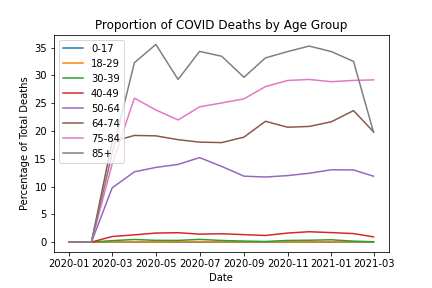
\includegraphics[scale=0.55]{"../figures/death_proportions_by_age.png"}
\caption{COVID Deaths by Age Group}
\end{wrapfigure}
The second data set, created and maintained by CDC \href{https://data.cdc.gov/NCHS/Provisional-COVID-19-Deaths-by-Sex-and-Age/9bhg-hcku}{here}, contains statistics of death counts by COVID-19 broken down by state, month, sex, and age group (among other data). For our analysis we took the smallest granularity, monthly, and focused on age groupings for each state. Since the age groupings overlapped, we restricted to looking at the following disjoint bins:  0-17,  18-29, 30-39, 40-49, 50-64, 65-74, 75-84, and 85 years and over. We first filled NA's, and took sums across these bins to compute the proportion of deaths accounted for by each age group (within the state, year, and month groupings)\footnote{For columns where the total across all ages was 0, a proportion of zero was given to all age groups.}.  In Figure 1 we see that, as expected, older age groups accounted for much larger proportions of deaths. 

%/figures/death_proportions_by_age.png



\newpage
\subsubsection{Weather Data}
The weather data was obtained from NOAA, the National Oceanic and Atmospheric Administration, which maintains monthly data of recorded temperatures by "Division" (subsets of states). The data source can be found \href{https://www.ncdc.noaa.gov/cag/divisional/mapping/110/tavg/202010/ytd/value}{here}. While the data here are spatially more granular than the COVID case data, with multiple divisions per state, it is less granular temporally, with temperature values per month only. Furthermore, NOAA does not include the District of Columbia as a Division, so this region is excluded from the weather modeling analysis. The weather data range from late 1800s to 2021, covering the range of dates found in the COVID cases data. 

Since global warming has seen a positive trend in temperatures,  as demonstrated by Figure 2 below, only the weather data from the last two decades (2000-2021) were included for analysis.
 
\begin{figure}[h]
\centering
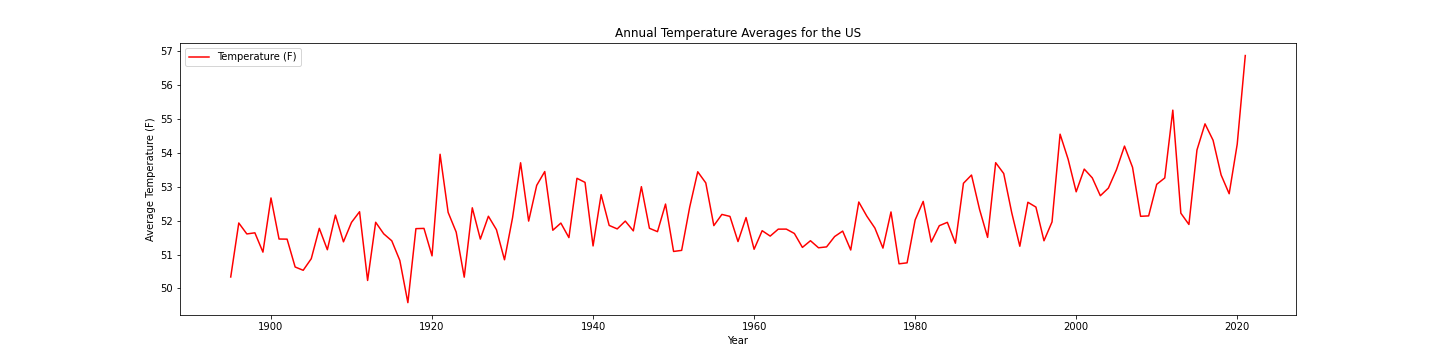
\includegraphics[scale=0.35]{"../figures/global_warming.png"}
\caption{Annual average state temperatures in the US from 1895 to 2021. }
\end{figure}


\begin{wrapfigure}{R}{0.5\textwidth}
\centering
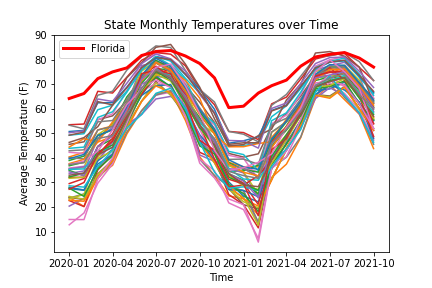
\includegraphics[scale=0.55]{"../figures/state_month_temps_FL.png"}
\caption{State temperatures (F) over time.}
\end{wrapfigure}
The state name was extracted from the Division names using regular expressions, and the date, stored in YYYYMM format, was parsed into month and year columns. Next, to obtain a single metric for each state (with a given month and year), the data were grouped by state and aggregate by taking an average of the temperatures. For the time range in which we have COVID data, these monthly averages are plotted for each state in Figure 3.  Florida is highlighted as a clear outlier in its monthly weather temperatures, remaining closer to moderate year-round. 

From the weather data, baseline monthly average were compute from recent historical values (2000-2019), and monthly averages per state were computed for the months during the pandemic (April 2020 to March 2021). Finally, when this data was merged with finer granularity data (e.g. daily), the monthly values were assigned to all days within the given month. This does allow for some ``future data leakage" when current monthly averages are fed into a model which incorporates implicit weather data from later in the month. Given more time, this would have been handled by computing an `expected monthly average` by taking the previous month's average, computing a delta from the recent historical average for that month, and adding that same delta to the historical average for the current month. 

%
%\subsubsection{Vaccination Data}
%The CDC maintains a database of vaccination data. 


\subsection{Causal Inference}
%a brief overview of causal inference, which should be written in a way such that another student in Data 100 who has never been exposed to the concept can carry out the analyses involving the datasets in your project.

A black-box forecasting model that can predict COVID-19 cases based on data that is measurable prior to the time of forecasting can be used in allocating resources for hospitals such as ventilators or health care workers as well as vaccines. However such a model would not provide any underlying information about the \textit{causes} of spikes in case number and may be limited in the public health policy ramifications. 

In contrast, an interpretable forecasting model would provide future estimates as well as inference into the underlying factors that influence the spread of the virus or its fatality. A feature of a linear model will have an impact on the outcome if its coefficient in the model differs from 0, which would represent excluding the feature from the model. Given training data, a linear model can be fit and the coefficients determined for each feature. However variability in sampling as well as co-linearity can confound the effects of a feature, either by yielding an non-zero coefficient for an irrelevant feature or by weighting an influential feature with a close to zero coefficient, so we turn to bootstrapping methods to create confidence intervals for these coefficients. 

Bootstrapping is based on the idea of resampling. If we had access to the overall population and could resample arbitrarily many times, we could construct numerous samples, and for each fit a linear model and look at the range of coefficients for each feature across the samples. A feature that significantly affects the outcome in the underlying population will yield a significant coefficient most of the time, although randomness may prevent it from being so in all samples. While this is unrealistic, if we can plausibly assume our sample is representative of the overall population, then we can perform a similar resampling method \textit{on our sample}, and create confidence intervals for our coefficients using the resampled models.  

One final issue that must be considered when attempting to infer causality from a linear model is the issue of colinearity. The meaning of a coefficient in a linear model is the effect of that feature \textit{while holding all others constant}. In the case that two or more features are linearly dependent, i.e. one can be expressed as a linear combination of the others, then it will be impossible to vary one without changing the others as well according to their linear relationship. Thus interpreting the coefficient becomes meaningless. For example with two features that are multiples of each other, slight changes in the data could result in one feature having a positive coefficient and the other with a near-zero coefficient, while a different model may reverse these effects. As a result, the confidence intervals for \textit{both} coefficients are likely to contain zero, since each variable is masking the effect of the other across different models. 

%\todo{ADD CAUSAL INFERENCE REMARKS FOR MY MODEL(S)!!}

%write up "causal inference" for modeling, i.e. bootstrapping confidence intervals for coefficients and what that means. 


%https://data102.org/sp20/assets/notes/notes13.pdf

%want to determine effects... 
%but can have confounding effects (example with graphs) 
%want to control for these confounding variables, but not mediators (intermediate variables creating a pathway of effect from one variable to another). 

%Can hold constant confounding variables and look at the effects within this population? 




\subsection{Forecast Modeling}


The first research aim involves a forecast modeling component, creating a baseline model and then incorporating particular features into the model and comparing performance. When training and interpreting forecasting models, it is important to consider the aim of the model in its construction. There are two types of forecasting models: ex-ante and ex-post. In an ex-ante model, the forecast should aim to predict \textit{future} outcomes, using only data up to the moment a forecast is made. In a ex-post model, any data may be used, including future data. In this case the model will not have true \textit{predictive} power, since making a future prediction will require future data first. However such models can be useful for interpreting relationships. 
In this research, we would like our models to have predictive capabilities and thus stick to ex-ante models. 
%
To avoid leaking the `future' into training, we must split our data in a temporal fashion\footnote{rather than taking random subsets of dates or even random subsets of states}. The primary data has daily entries for a span of twelve months, ten of which are used for training and one each for validation and testing. 

% 
%ex-ante vs post-ante forecasting article:\\
%https://otexts.com/fpp2/forecasting-regression.html\#ex-ante-versus-ex-post-forecasts
%%

\subsubsection{Weather Modeling}


\begin{wrapfigure}{R}{0.4\textwidth}
\centering
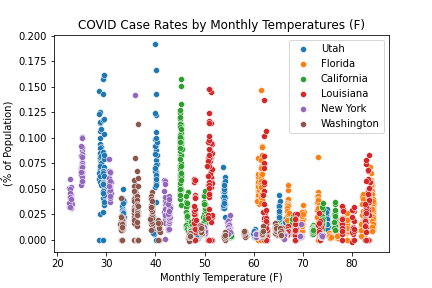
\includegraphics[scale=0.45]{"../figures/case_rates_by_temp.png"}
\caption{Case rates by temperature.}
\end{wrapfigure}
Over the course of the pandemic, scientists have realized that COVID transmission is low in outdoor settings, but indoors exposure maintains a high risk of infection. During warm months, people can easily adhere to outdoor only gatherings, but during particularly hot or cold weather, people are more likely to gather indoors, thus increasing possible exposure. 

After computing daily counts for new confirmed cases and taking these as a proportion of the total state population, we grouped the case rates by the temperature of the month in which they occurred and plotted these clusters for several states (Figure 4).

For each state shown, we see that lower temperatures have wider spreads of case rates, and in particular contain the highest values for each state. One interesting note is that these `cold weather effects' occur at different temperatures for different states. For example, California (in green) sees a spike in case rates around 45-50 degrees, whereas Washington maintains fairly low rates in that range, but sees increases at 40 degrees and below. On the other end of the spectrum, Louisiana, a warmer state, sees potential `cold weather` spikes as high as 60 degrees. 

This difference between states is easily understood since what may feel `cold' varies depending on state norms and average temperatures. Washington is a colder state than California which in turn is colder than Louisiana. To incorporate this effect into our data then, we computed for each entry how far below the recorded temperature was from the state's annual average temperature, taking a value of 0 when the recorded temperature was higher (selecting on `cold' deviations). This metric was then fed into the model both as a raw entry in addition to case data, and as a multiplier for the existing case rates. 

A baseline model was first trained using recent daily confirmed case rates, from the past 14 days (the length of possible COVID incubation). 
Each weather variant of the model was then given additional features from weather data and trained on all states in the training data. Since the model is fed state level data, it is trained to make predictions on a state level. Thus to measure the models accuracy, we compute \textit{for each state} the root mean-squared error (RSME) on each data set and then averaged the state RSMEs to get a single metric. 

\subsubsection{Death by Age Analysis}

To analyze patterns in death statistics by state, we took the data set containing deaths by age group by state and month, and created larger age bins: 0-29 years, 30-64 years, and 65 years and older. The values for each column represented the proportion of COVID-19 deaths that month belonging to the specified age group (within a given state). This was then pivoted so that for each state, there was a column for each month and age group pair. This data was then standardized and singular valued decomposition was used to extract the principal components. 

Initially the data for this PCA spanned from April 2020 to March 2021. However given the start of the vaccine roll out in early 2021, a secondary analysis split the deaths data into two clusters, by year and repeated the same principal component analysis on each year. 


\newpage

\section{Results}

 
%Analysis of your findings to answer your research question(s). Include visualizations and specific results. If your research questions contain a modeling component, you must compare the results using different inference or prediction methods (e.g., linear regression, logistic regression, or classification and regression trees). Can you explain why some methods performed better than others?


\subsection{Weather Modeling}

To evaluate the potential effect of cold weather on COVID transmission, we first trained a baseline forecasting model which took as input the confirmed daily cases for the past 14 days for a given state, and tried to predict the daily case rate for the next day. Notably, this model (Model 1 below) saw a significantly \textit{lower} average state RSME on the validation set than on the training set. One possible explanation for this is the temporal nature of the data, such that the training data covers ten months, while the validation set only spans a single month. As a result, an increased variability in case numbers over the first ten months may be due to factors not captured by the data (variants, holiday travel, masking/social distancing policies, etc). As a result, the model has higher error on the training set, despite training on that same data. Since this trend persists throughout all the models considered for this section, it does not impact our analysis or our ability to compare models.

\begin{figure}[h]
\centering
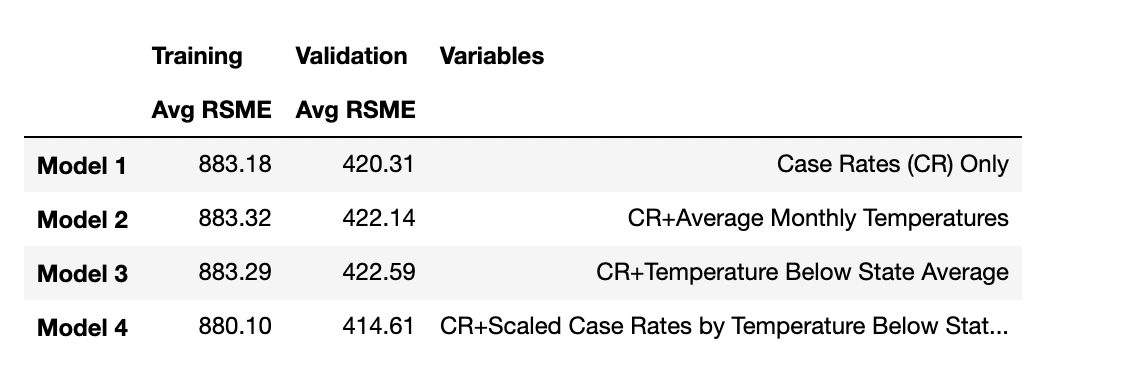
\includegraphics[scale=0.75]{"../figures/weather_model_report.png"}
\caption{Model Performance Metrics for Weather Models}
\end{figure}

Next, the average monthly temperatures for each state we combined with the confirmed case data and fed into a new linear model. Since temperature ranges vary by state and both hot and cold extremes are suspected to cause increases, this variable was not expected to improve the model performance significantly. Indeed, this model (Model 2 below) sees a similar average RSME on the training set, and actually a slightly higher average RSME on the validation set. 

The next two models incorporate the computed metric of how far below the state's annual average temperature a given monthly average is. Model 3 incorporates this value as its own feature in the model, while Model 4 scales the cases for the last 14 days by this value (original case numbers are retained in the model as well, since temperatures at or above average have a computed scaling term of 0). 

While Model 3 performs similarly to the previous two models, Model 4, which has the scaled numbers, sees a slight increase on the training set and a larger increase on the validation set. Notably, the effects are not as pronounced as Figure 4 suggested. If colder weather does cause an increase in case transmissions, this might be on a larger time scale than 2 weeks, which is not captured by any of the weather models above. However to the extent that recent weather does affect transmission, the effect might be mediated by the recent case numbers already used by the model which were likely subject to similar temperatures. With only a year of data, and temperatures reported \textit{monthly}, there may not be enough granularity for the model to pick up on temperature sensitivity. 





\subsection{Death by Age Modeling}

\begin{wrapfigure}{R}{0.4\textwidth}
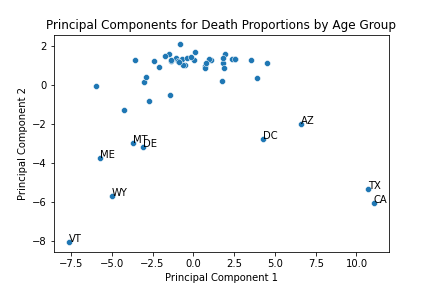
\includegraphics[scale=0.5]{"../figures/initial_death_pca.png"}
\caption{Deaths Age Distribution PCA}
\end{wrapfigure}
The results of the first two principal components for each state\footnote{still only considering continental US states and the District of Columbia} from PCA on the death proportions by age for the months of April 2020 to March 2021 are shown in Figure 6. The first principal component accounts for approximately 35\% of the variance, while the second accounts for 15\%. We see from the scatter plot that most states are clustered in an oval cloud, with two strands of outliers to the lower left and lower right (labeled). The two states with the higher PC1 values are Texas and California, which are also the states with the highest populations in the United States. In contrast, Minnesota, Vermont, and Wyoming are much less densely populated. Since COVID spikes (and thus likely deaths) are prevalent in heavily populated cities, this first principal component might be capturing a ``population density" metric for the states. We also see that the District of Columbia appears as an outlier here, which seems reasonable since it is the only city represented in the dataset. 

Next we want to split the months into pre and post vaccine sets and perform the same PCA analysis for each. Vaccine roll-out began in early 2021, so the pre-vaccine months are taken to be all of those in 2020 and the post-vaccine months (which capture only the beginning of the effects of vaccination) are January through March of 2021. The results for the first two components of each PCA are shown below. 


\begin{figure}[h]
\centering
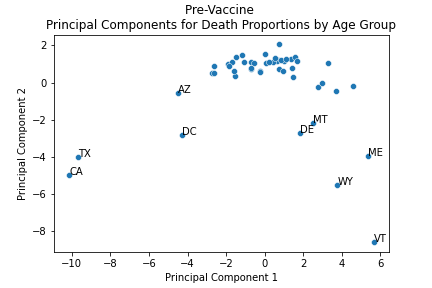
\includegraphics[scale=0.45]{"../figures/pre_vaccine_death_pca.png"}
%\end{figure}
%
%\begin{figure}[h]
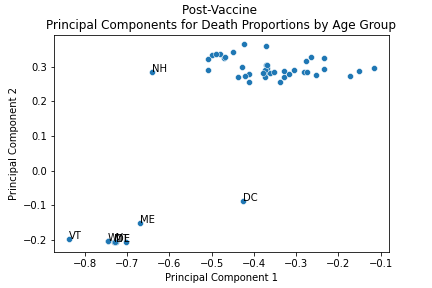
\includegraphics[scale=0.45]{"../figures/post_vaccine_death_pca.png"}
\caption{Pre- and Post-Vaccine Deaths Age Distribution PCA}
\end{figure}

For pre-vaccine data, the first two principal components capture 31\% and 16\% variance, compared to the post-vaccine data, where they account for 59\% and 17\% of the variance. In the pre-vaccine PCA, we see a picture very similar to our initial analyses, although reflected and slightly rotated. This is not surprising as the pre-vaccine data accounts for three quarters of the data used for the first. However when we examine post-vaccine data by itself, we get a drastically different picture. In this figure we see a large oval cluster of states with positive PC2 and larger PC1, with a small tight knit cluster in the lower left (negative PC2 and small PC1). The small cluster includes the states Delaware, Maine, Montana, North Carolina, North Dakota, South Dakota, and Vermont. These states have (relatively) low and dispersed populations, but saw vaccinations rise quickly once available (compared to more vaccine hesitant states). 

%\subsection{Limitations and Future Research}
% An evaluation of your approach and discuss any limitations of the methods you used.

%Describe any surprising discoveries that you made and future work.

%\subsection{Future Research}



%--/Paper--

\end{document}